\section{Hardware Oriented Model Compression}\label{sec:software}

As introduced in section~\ref{sec:design_method}, the design of energy efficient and fast neural network accelerator can benefit from the optimization of NN models. A larger NN model usually results in higher model accuracy. This means it is possible to trade the model accuracy for the hardware speed or energy cost. Neural network researchers are designing more efficient network models from AlexNet~\cite{krizhevsky2012imagenet} to ResNet~\cite{he2016deep}, SqueezeNet~\cite{iandola2016squeezenet} and MobileNet~\cite{Howard2017MobileNets}. The main differences between these networks are the size of and the connections between each layer. The basic operations are the same and hardly affect the hardware design. For this reason, we will not focus on these techniques in this paper. Other methods try to achieve the tradeoff by compressing existing NN models. They try to reduce the number of weights or reduce the number of bits used for each activation or weight, which help lower down the computation and storage complexity. Corresponding hardware designs can benefit from these NN model compression methods. In this section, we investigate these hardware oriented network model compression methods.

\subsection{Data Quantization}\label{sec:software:quant}
One of the most commonly used methods for model compression is the quantization of the weights and activations. The activations and weights of a neural network are usually represented by floating point data in common developing frameworks. Recent work tries to replace this representation with low-bit fixed-point data or even a small set of trained values. On the one hand, using fewer bits for each activation or weight helps reduce the bandwidth and storage requirement of the neural network processing system. On the other hand, using a simplified representation reduce the hardware cost for each operation. The benefit of hardware will be discussed in detail in section~\ref{sec:hardware}. Two kinds of quantization methods are discussed in this section: linear quantization and non-linear quantization.

\subsubsection{Linear Quantization}
Linear quantization finds the nearest fixed-point representation of each weight and activation. The problem with this method is that the dynamic range of floating-point data greatly exceeds that for fixed-point data. Most of the weights and activations will suffer from overflow or underflow. Qiu et al.~\cite{qiu2016going} finds that the dynamic range of the weights and activations in a single layer is much more limited and differs across different layers. Therefore they assign different fractional bit-widths to the weights and activations in different layers. To decide the fractional bit-width of a set of data, i.e. the activations or weights of a layer, the data distribution is first analyzed. A set of possible fractional bit-widths are chosen as candidate solutions. Then the solution with the best model performance on training data set is chosen. In~\cite{qiu2016going}, the optimized solution of a network is chosen layer by layer to avoid an exponential design space exploration. Wang et al.~\cite{wang2018design} try to use large bit-width for only the first and last layer and quantize the middle layers to ternary or binary. The method needs to increase the network size to keep high accuracy but still brings hardware performance improvement.  Guo et al.~\cite{guo2017angel} choose to fine-tune the model after the fractional bit-width of all the layers are fixed.  

The method of choosing a fractional bit-width equals to scale the data with a scaling factor of $2^k$. Li et al.~\cite{li2016ternary} scales the weights with trained parameter $W^l$ for each layer and quantize the weights with 2-bit data, representing $W^l$, 0 and $-W^l$. The activations in this work are not quantized. So the network still implements 32-bit floating point operations. Zhou et al.~\cite{zhou2016dorefa} further quantize the weights of a layer with only 1 bit to $\pm s$, where $s=E(|w^l|)$ is the expectation of the absolute value of the weights of this layer. Linear quantization is also applied to the activations in this work.

\subsubsection{Non-linear Quantization}
Compared with linear quantization, non-linear quantization independently assigns values to different binary codes. The translation from a non-linear quantized code to its corresponding value is thus a look-up table. This kind of methods helps further reduce the bit-width used for each activation or weight. Chen et al.~\cite{chen2015compressing} assign each of the weight to an item in the look-up table by a pre-defined hash function and train the values in look-up tables. Han et al.~\cite{han2015deep} assign the values in look-up tables to the weights by clustering the weights of a trained model. Each look-up table value is set as the cluster centre and further fine-tuned with training data set. This method can compress the weights of state-of-the-art CNN models to 4-bit without accuracy loss. Zhu et al.~\cite{zhu2016trained} propose the ternary-quantized network where all the weights of a layer are quantized to three values: $W^n$, 0, and $W^p$. Both the quantized value and the correspondence between weights and look-up table are trained. This method sacrifices less than $2\%$ accuracy loss on ImageNet dataset on state-of-the-art network models. The weight bit-width is reduced from 32-bit to 2-bit, which means about $16\times$ model size compression.

\subsubsection{Comparison}
\begin{figure}[ht]
    \centering
    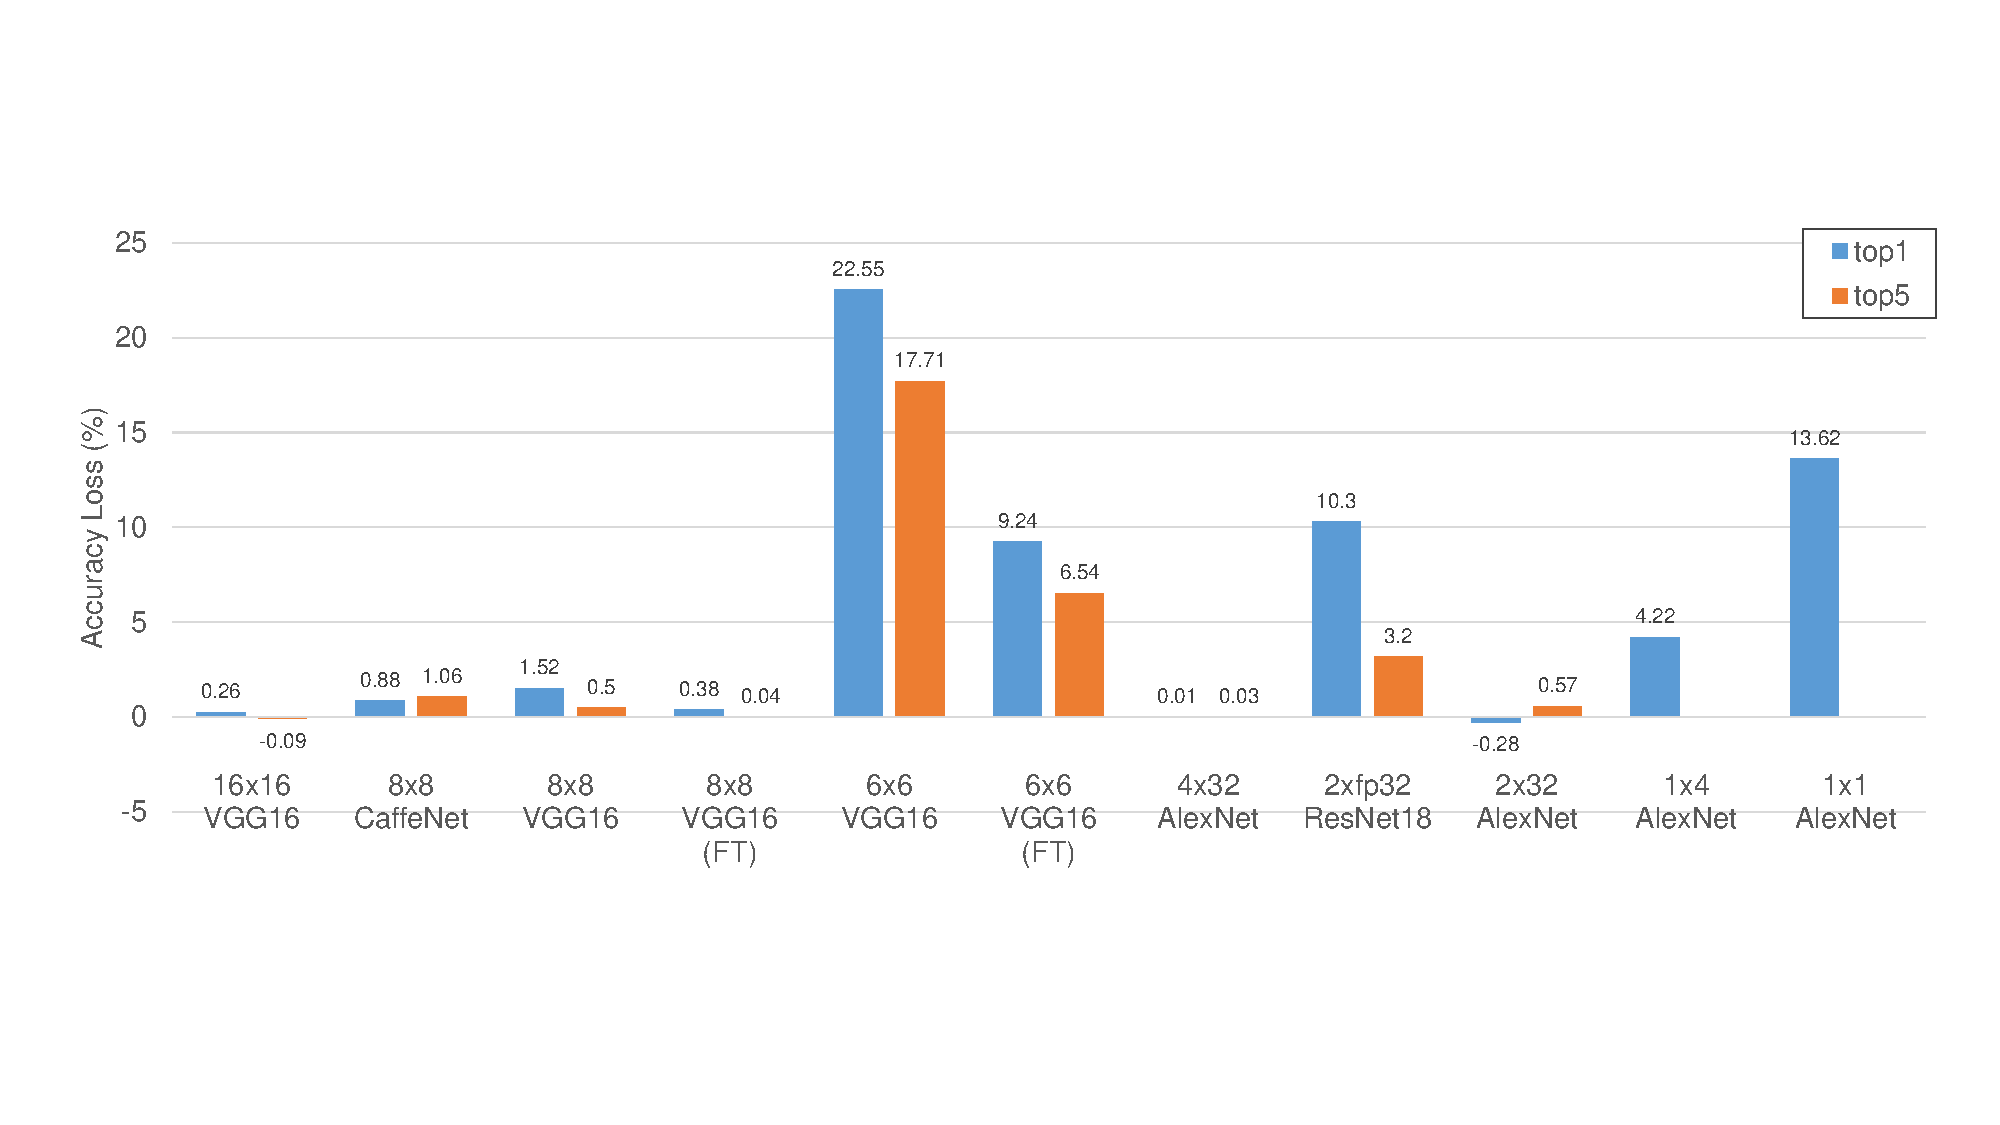
\includegraphics[width=1.0\columnwidth]{fig/quantization.pdf}
    \caption{Comparison between different quantization methods from \cite{qiu2016going, guo2017angel, han2015deep, zhu2016trained, zhou2016dorefa, li2016ternary}. The quantization configuration is expressed as (weight bit-width)$\times$(activation bit-width). The "(FT)" denotes that the network is fine-tuned after a linear quantization.}
    \label{fig:quantization}
\end{figure}

We compare some typical quantization methods from~\cite{qiu2016going, guo2017angel, han2015deep, zhu2016trained, zhou2016dorefa, li2016ternary} in Figure~\ref{fig:quantization}. All the quantization results are tested on ImageNet data set and the absolute accuracy loss compared with corresponding baseline floating point models is recorded. Comparing different methods on different models is a little bit unfair. But it still gives some insights. For linear quantization, 8-bit is a clear bound to ensure negligible accuracy loss. With 6 or fewer bits, using fine-tune or even training each weight from the beginning will cause noticeable accuracy degradation. If we require that $1\%$ accuracy loss is within the acceptable range, linear quantization with at least $8\times 8$ configuration and the listed non-linear quantization are available. We will further discuss the performance gain of quantization in section~\ref{sec:hardware}. 


\subsection{Weight Reduction}\label{sec:software:wr}
Besides narrowing the bit-width of activations and weights, another method for model compression is to reduce the number of weights. One kind of method is to approximate the weight matrix with a low-rank representation. Qiu et al.~\cite{qiu2016going} compress the weight matrix $W$ of an FC layer with singular value decomposition. An $m\times n$ weight matrix $W$ is replaced by the multiplication of two matrices $A_{m\times p}B_{p\times n}$. For a sufficiently small $p$, the total number of weights is reduced. This work compresses the largest FC layer of VGG network to $36\%$ of its original size with $0.04\%$ classification accuracy degradation. Zhang et al.~\cite{zhang2015efficient} use a similar method for convolution layers and takes the effect of the following non-linear layer into the decomposition optimization process. The proposed method achieves $4\times$ speed up on state-of-the-art CNN model targeting at ImageNet, with only $0.9\%$ accuracy loss.

Pruning is another kind of method to reduce the number of weights. This kind of methods directly remove the zeros in weights or remove those with small absolute values. The challenge in pruning is the tradeoff between the ratio of zero weights and the model accuracy. One solution is the application of lasso method, which applies L1 normalization to the weights during training. Liu et al.~\cite{liu2015sparse} apply the sparse group-lasso method on the AlexNet~\cite{krizhevsky2012imagenet} model. $90\%$ weights are removed after training with less than $1\%$ accuracy loss. Another solution is to prune the zero weights during training. Han et al.~\cite{han2015deep} directly remove the weights of a network which are zero or have small absolute value. The left weights are then fine-tuned with the training dataset to recover accuracy. Experimental results on AlexNet show that $89\%$ weights can be removed while keeping the model accuracy.

The hardware gain from weight reduction is the reciprocal of the compression ratio. According to the above results, the improvement from weight reduction is up to $10\times$.